\documentclass[11pt,a4paper]{article}
\usepackage{fontspec}
\setmainfont{cmunrm.otf}[BoldFont=cmunbx.otf,ItalicFont=cmunti.otf,BoldItalicFont=cmunbi.otf]
\usepackage[english,russian]{babel}
\usepackage[margin=24mm,top=20mm,bottom=22mm]{geometry}
\usepackage{amsmath,amssymb,booktabs,graphicx,caption,microtype}
\usepackage[unicode,hidelinks]{hyperref}
\hypersetup{pdftitle={Рассеяние волн при переменных коэффициентах среды}}
\captionsetup{font=small,labelfont=bf,labelsep=period}
\setlength{\parindent}{1.25em}
\setlength{\emergencystretch}{1.2em}
\newcommand{\ii}{\mathrm{i}}
\newcommand{\R}{\mathbb R}
\newcommand{\C}{\mathbb C}
\newcommand{\T}{\mathsf T}
\newcommand{\norm}[1]{\lVert #1\rVert}
\newenvironment{localtable}{\par\medskip\begingroup\centering\small\renewcommand{\arraystretch}{1.18}}{\par\endgroup\medskip}
\newenvironment{localfigure}{\par\smallskip\begingroup\centering}{\par\endgroup\smallskip}
\makeatletter
\newcommand{\tabinput}[1]{\@@input #1.tex }
\makeatother
\newcommand{\BestRank}{24}
\newcommand{\BestMean}{0,86}
\newcommand{\BlindMean}{33,33}
\newcommand{\BestFloor}{0,15}
\newcommand{\GmsMean}{0,26}
\newcommand{\BestMedian}{0,80}
\newcommand{\BestTail}{1,35}
\newcommand{\WidthSmall}{1,40}
\newcommand{\WidthLarge}{0,99}
\newcommand{\Wins}{128}
\newcommand{\AlphaTrue}{9,09}
\newcommand{\AlphaPred}{8,95}
\newcommand{\AlphaError}{13,90}
\newcommand{\IndexTrue}{45,64}
\newcommand{\IndexPred}{45,56}
\newcommand{\IndexError}{2,14}

\begin{document}
\begin{center}
{\Large\bfseries Рассеяние волн при переменных коэффициентах среды: приближение методами SVD-SNO и GMsFEM\par}
\end{center}

\noindent\textbf{Аннотация.}
Рассматривается рассеяние плоской волны на двух группах проницаемых включений. Коэффициент при градиенте и коэффициент при волновом члене изменяются в каждой группе. Для 160 сред рассчитаны 1\,280 полей МКЭ. По четырём параметрам материала и направлению волны восстанавливаются коэффициенты поля в базисе снимков. На 16 отложенных средах средняя относительная погрешность спектрального нейрооператора составила \BestMean\%, при исключении материальных параметров из входа получено \BlindMean\%. Для многомасштабного метода с 16 локальными модами типа~2 получено \GmsMean\%. В отдельной серии измерена погрешность приращения поля при поочерёдном изменении двух коэффициентов.

\smallskip\noindent\textbf{Ключевые слова:} уравнение Гельмгольца, рассеяние волн, коэффициенты среды, метод конечных элементов, сингулярное разложение, спектральный нейрооператор.

\section*{Введение}
Замена материала включения меняет амплитуду и фазу рассеянной волны. Чтобы определить эту зависимость по снимкам решения, будем изменять коэффициенты внутри включений при фиксированных геометрии и волновом числе. Исследуем точность прогноза для новых сред и отдельно оценим, как сеть воспроизводит приращение поля при изменении одного коэффициента.

\section{Постановка задачи}
Пусть $\Omega=(-2,2)^2$. Обозначим через $D_1$ объединение 19 кругов радиусов $0{,}02$ и $0{,}05$, а через $D_2$ объединение пяти кругов радиуса $0{,}10$. Для изотропной среды положим $A(x)=a(x)I$. Во включениях $D_j$ зададим $a(x)=a_j$, $n(x)=n_j$, а в фоне $a(x)=n(x)=1$. Таким образом, одна среда определяется вектором
\[
 p=(a_1,a_2,n_1,n_2),\qquad 0{,}4\le a_j\le0{,}9,\quad 2\le n_j\le6.
\]
Для падающей волны $u_i(x)=\exp(\ii k d\cdot x)$, $d=(\cos\theta,\sin\theta)$, $k=2$, требуется найти рассеянное поле $u_s$ такое, что
\begin{equation}
 \nabla\!\cdot(A\nabla u)+k^2nu=0\quad\text{в }\Omega,\qquad
 (A\nabla u_s)\cdot\nu-\ii k u_s=0\quad\text{на }\partial\Omega,\quad u=u_i+u_s .
 \label{eq:pde}
\end{equation}
Здесь $\nu$ обозначает внешнюю нормаль. На границах включений непрерывны полное поле и нормальная компонента потока $A\nabla u$. На внешней границе используется поглощающее условие первого порядка.
\begin{localfigure}
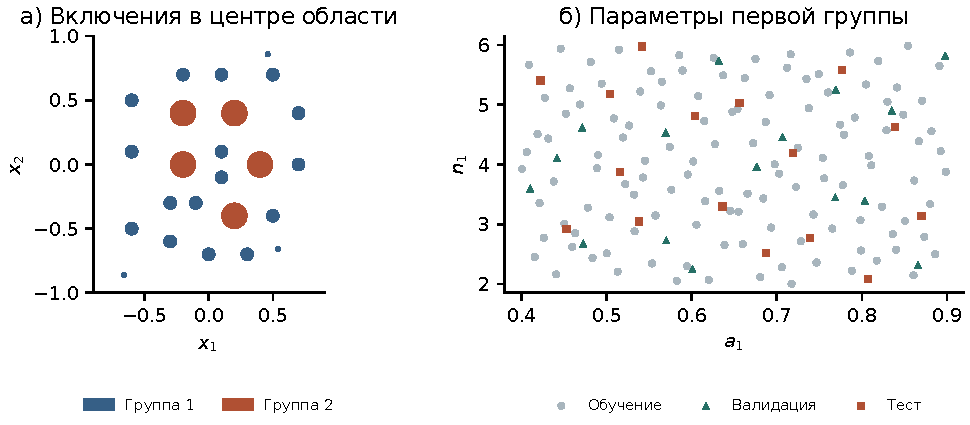
\includegraphics[width=.69\linewidth]{figures/design.pdf}
\captionof{figure}{Две группы круговых включений и проекция выборок на плоскость $(a_1,n_1)$. Каждая точка правого рисунка соответствует одной среде.}
\end{localfigure}

\clearpage
\section{Метод конечных элементов}
На треугольной сетке, согласованной с границами кругов, введём пространство $V_h\subset H^1(\Omega;\C)$ непрерывных кусочно-линейных функций. Подставим $u=u_i+u_s$ в~\eqref{eq:pde} и воспользуемся уравнением для падающей волны в однородном фоне. После интегрирования по частям получим задачу: найти приближение $u_h\in V_h$ рассеянного поля, удовлетворяющее для всех $v_h\in V_h$ равенству
\begin{align}
 \int_\Omega a\nabla u_h\cdot\nabla\overline v_h\,dx-k^2\int_\Omega n u_h\overline v_h\,dx
       -\ii k\int_{\partial\Omega}u_h\overline v_h\,ds
      ={}&\int_\Omega(1-a)\nabla u_i\cdot\nabla\overline v_h\,dx\nonumber\\
      &+ k^2\int_\Omega(n-1)u_i\overline v_h\,dx .\label{eq:weak}
\end{align}
Коэффициенты задаются по элементам. Из~\eqref{eq:weak} видно, что $a_j$ входит в матрицу жёсткости и градиентную часть нагрузки, а $n_j$ входит в матрицу масс и второе слагаемое нагрузки. При переходе к новой среде пересчитываются обе части системы
\begin{equation}
 H(p)U_h=F(p,\theta),\qquad H(p)=K_a-k^2 M_n-\ii k B ,
 \label{eq:fem}
\end{equation}
где $U_h$ есть вектор узловых значений $u_h$, а $B$ обозначает граничную матрицу масс. Эталонная сетка имеет заданный шаг $0{,}02$, 53\,246 узлов и 105\,690 треугольников. Для комплексного вектора $z$ введём $\norm{z}_M=(z^*Mz)^{1/2}$, где $M$ есть согласованная матрица масс с единичным весом. Эта норма совпадает с $L^2$-нормой соответствующей кусочно-линейной функции.

\subsection*{Многомасштабный метод конечных элементов}
Для сравнения применим GMsFEM в постановке для рассеяния волн~\cite{kalachikova}. Крупная сетка состоит из $20\times20$ квадратов. В окрестности крупной вершины $q$ решим локальные задачи на вспомогательной сетке с шагом $0{,}04$. В каждой задаче граничные данные равны единице в одном узле и нулю в остальных. В базисе типа~1 используется оператор $-\nabla\!\cdot(a\nabla)$, в базисе типа~2 учитывается также слагаемое $-k^2n$. Пусть $\Psi_q$ обозначает матрицу полученных локальных решений. Выберем первые $m$ собственных векторов в порядке возрастания собственных значений задачи
\[
 (\Psi_q^*K_{a,q}\Psi_q)v=\lambda(\Psi_q^*M_{a,q}\Psi_q)v.
\]
Здесь вес локальной матрицы масс равен $a$. После умножения локальных мод на вершинные функции, полученные локальным продолжением билинейных граничных следов, получим матрицу базиса $P$. Решается система $(P^*H_{0{,}04}P)y=P^*F_{0{,}04}$ размера $441m$. Для каждой из 16 тестовых сред строится свой базис каждого типа. В пределах одной среды базис и матрица Галёркина используются для восьми направлений.

\section{Метод сингулярного разложения (SVD)}
Для действительной и мнимой частей $U_h$ построим отдельные базисы по обучающим снимкам. Пусть строки $X$ есть центрированные узловые значения одной из компонент, а $\bar f$ есть её среднее по обучающей выборке. В методе снимков~\cite{sirovich} пространственные моды определяются из равенств
\begin{equation}
 XMX^\T v_j=\sigma_j^2v_j,\qquad \phi_j=X^\T v_j/\sigma_j,\qquad
 \Phi_r^\T M\Phi_r=I_r,\qquad \Phi_r=(\phi_1,\ldots,\phi_r).
 \label{eq:svd}
\end{equation}
Для нового поля $f$ коэффициенты равны $c=\Phi_r^\T M(f-\bar f)$, его проекция равна $\bar f+\Phi_r c$. Для комплексного решения сохраняются $2r$ вещественных коэффициентов. Входные поля материала полностью задаются четырьмя числами $p$, поэтому для них отдельное сингулярное разложение не требуется.

\clearpage
\section{Метод спектрального нейрооператора (SNO)}
В спектральном представлении~\cite{fanaskov} нейросеть действует на конечную таблицу коэффициентов. В нашей задаче пространственный базис выхода определяется по~\eqref{eq:svd}, а на вход подаются значения материала и параметры волны. Каждая координата $p$ нормируется по своему среднему и стандартному отклонению на обучающей выборке. Обозначим полученные числа через $\widetilde a_j,\widetilde n_j$. Для $j=1,2$ входная строка равна
\[
  (\widetilde a_j,\widetilde n_j,\cos\theta,\sin\theta,0).
\]
В строках $j=3,\ldots,r$ обе материальные компоненты равны нулю. Последняя компонента во всех строках равна нулю, так как $k$ фиксировано. Номер строки здесь служит для размещения входных данных: пространственные моды выхода определяются снимками и зависят от всей среды.

Линейный слой с активацией GELU переводит вход в таблицу $Z\in\R^{r\times w}$. В каждом из четырёх последовательных блоков вычисляется
\begin{equation}
 Z'= Z+\operatorname{GELU}(ZW_1+\mathbf1b^\T + DZW_2).
 \label{eq:block}
\end{equation}
Матрица $D$ смешивает $r$ мод, а $W_1,W_2$ действуют по $w$ признакам. Линейный выходной слой даёт по два числа на моду. После умножения на обучающие стандартные отклонения коэффициентов восстанавливаются действительная и мнимая части поля. Число обучаемых параметров равно $P=4(2w^2+w+r^2)+8w+2$.
\begin{localfigure}
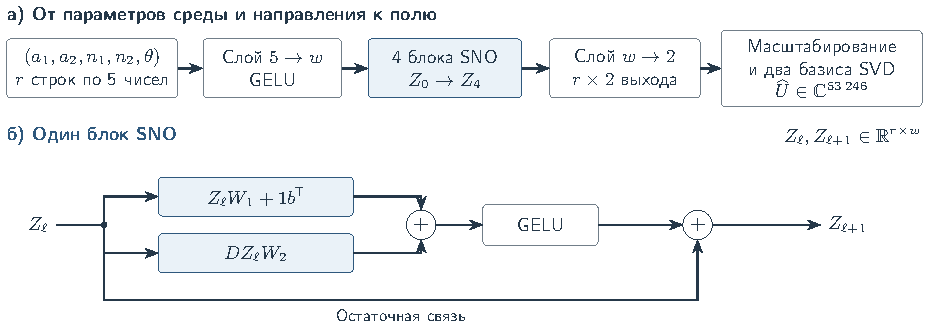
\includegraphics[width=.94\linewidth]{figures/architecture.pdf}
\captionof{figure}{Архитектура SVD-SNO для переменной среды. Материальные параметры поступают в первые две строки таблицы, а матрица $D$ связывает эти строки с остальными модами.}
\end{localfigure}

\section{Вычислительная реализация}
Для задания параметров в четырёхмерном прямоугольнике использована перемешанная последовательность Соболя~\cite{sobol}. Использованы первые 157 точек. Первые 125 сред образуют обучающую выборку, следующие 16 используются для выбора весов и ещё 16 для тестирования. Для каждой среды заданы восемь углов $\theta_j=(j+1/2)\pi/4$, $j=0,\ldots,7$. Подвыборки из 400, 600, 800 и 1\,000 полей вложены и содержат целые группы по восемь направлений. Ещё три специально заданные среды используются для проверки приращений. Всего решено 1\,280 задач~\eqref{eq:fem}.

Нумерация узлов считывается средствами DOLFINx. Правая часть вычисляется с квадратурой $8\times8$ на преобразованном треугольнике. Для каждой среды выполняется одна разреженная LU-факторизация и решаются восемь систем с одной матрицей. Максимальная относительная невязка составила $4{,}47\cdot10^{-13}$. Для оценки GMsFEM решение со вспомогательной сетки интерполируется в узлы эталона.

\clearpage
\section{Численные эксперименты}
Для каждой тестовой пары $(p,\theta)$ вычислим относительную погрешность комплексного рассеянного поля
\begin{equation}
 e(\widehat U)=100\,\norm{\widehat U-U_h}_M/\norm{U_h}_M .
 \label{eq:error}
\end{equation}
Средняя тестовая погрешность вычисляется как среднее арифметическое 128 значений этой величины. Благодаря ортогональности~\eqref{eq:svd} квадрат нормы разности равен сумме квадрата погрешности проекции и квадратов погрешностей $2r$ коэффициентов. По этому тождеству сеть обучается в пространстве коэффициентов с функцией потерь, равной среднему $e/100$ по пакету. Использован AdamW, размер пакета 64, начальный шаг $0{,}002$, конечный $0{,}00015$, косинусное расписание на 300 эпох, коэффициент убывания весов $10^{-5}$. Для каждого запуска начальное число генератора равно 2026. Веса выбираются по минимуму средней валидационной погрешности.

\subsection*{Размер выборки, число мод и ширина сети}
В табл.~\ref{tab:size} сравниваются три ранга при одной ширине $w=48$. Каждый раз базисы решения и нормировки определяются заново по соответствующему обучающему набору. При одном числе эпох число обновлений весов за эпоху растёт с размером выборки. В табл.~\ref{tab:rank} отдельно указана погрешность наилучшего восстановления поля в выбранном базисе.
\begin{localtable}
\captionof{table}{Средняя тестовая погрешность SVD-SNO при $w=48$, \%. Ранг указан для одной вещественной компоненты поля}\label{tab:size}
\begin{tabular}{rrrrr}\toprule Обучающих полей & Обучающих сред & $r=8$ & $r=16$ & $r=24$\\\midrule
\tabinput{tables/size}\bottomrule\end{tabular}
\end{localtable}
\begin{localtable}
\captionof{table}{Влияние базиса и числа обучаемых параметров $P$ при 1\,000 обучающих полях. Погрешности указаны в процентах}\label{tab:rank}
\begin{tabular}{lrrr rrrr}\toprule
Вход сети & $r$ & $w$ & $P$ & Проекция & Валидация & Тест & $q_{0{,}95}$\\\midrule
\tabinput{tables/rank}\bottomrule\end{tabular}
\end{localtable}

При $r=8$ увеличение выборки с 400 до 1\,000 полей снизило погрешность с 2,74 до 2,56\%, тогда как погрешность проекции осталась близкой к 2,5\%. При $r=24$ на тех же выборках получено 1,58 и 0,86\% соответственно. При $r=16$ изменение ширины с 24 до 48 даёт средние тестовые погрешности \WidthSmall\% и \WidthLarge\% соответственно. Для парного сравнения входных параметров выбран ранг $r=\BestRank$ по валидации среди трёх рангов при $w=48$. В той же архитектуре отдельно обучена сеть, которой доступно только направление волны. Базисы, число параметров и размер выборки обеих сетей совпадают. Без материальных данных получено \BlindMean\% средней погрешности, с материальными данными \BestMean\%. Погрешность проекции составляет \BestFloor\%.

\clearpage
\subsection*{Сопоставление с GMsFEM}
Для таблицы~\ref{tab:gms} все методы проверены на одних и тех же 128 задачах. Размер многомасштабной системы есть число комплексных неизвестных для одного решения. Параметры сети задают одно отображение для всей совокупности сред. Отдельный расчёт МКЭ с шагом $0{,}04$ показывает расхождение с эталонной сеткой до редукции многомасштабного пространства.
\begin{localtable}
\captionof{table}{Погрешность рассеянного поля на 16 тестовых средах, \%. Для GMsFEM $m$ обозначает число локальных мод на вершину}\label{tab:gms}
\begin{tabular}{lrrrrr}\toprule Метод & $m$ & Неизвестных & Средняя & Медиана & $q_{0{,}95}$\\\midrule
\tabinput{tables/gms}\bottomrule\end{tabular}
\end{localtable}

\begin{localfigure}
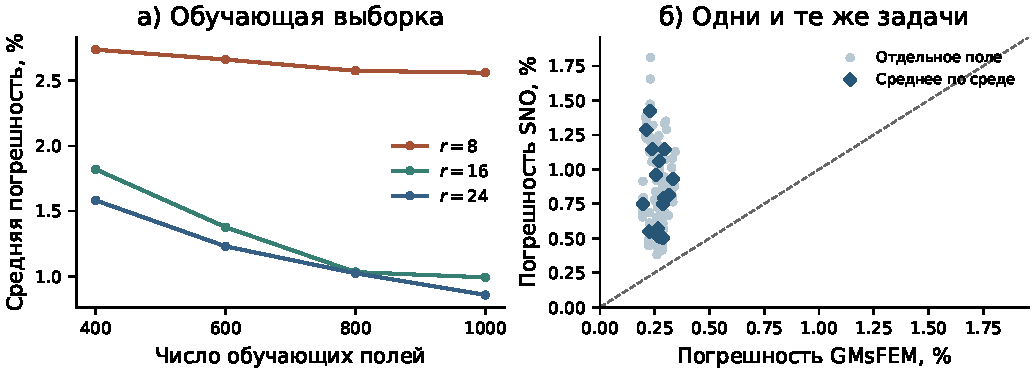
\includegraphics[width=.97\linewidth]{figures/paired.pdf}
\captionof{figure}{Слева приведена средняя тестовая погрешность при $w=48$. Справа сопоставлены GMsFEM типа~2 ($m=16$) и SVD-SNO ($r=\BestRank$, $w=48$, 1\,000 полей). Каждой среде соответствуют восемь задач. Точки ниже диагонали отвечают меньшей погрешности сети.}
\label{fig:paired}
\end{localfigure}
При увеличении числа локальных мод с 4 до 16 средняя погрешность типа~2 уменьшилась с 1,03 до 0,26\%. Для типа~1 соответствующие значения равны 1,53 и 0,31\%. На рис.~\ref{fig:paired} все 128 точек лежат выше диагонали. Полное решение МКЭ на вспомогательной сетке даёт в среднем 0,10\%.
\subsection*{Изменение одного коэффициента}
В качестве базовой среды возьмём $p_0=(0{,}45;0{,}65;2{,}4;4)$. В первой паре расчётов увеличим $a_1$ до $0{,}85$, во второй увеличим $n_1$ до $5{,}6$. В обоих случаях коэффициент изменяется во всех 19 включениях $D_1$. Для каждого угла найдём приращения $\Delta U_h=U_h(p,\theta)-U_h(p_0,\theta)$ и $\Delta\widehat U=\widehat U(p,\theta)-\widehat U(p_0,\theta)$. В табл.~\ref{tab:change} изменения МКЭ и SNO нормированы на норму собственного базового поля. В последнем столбце приведена погрешность самого приращения
\[
 E_\Delta=100\,\norm{\Delta\widehat U-\Delta U_h}_M/\norm{\Delta U_h}_M .
\]
\clearpage
\begin{localtable}
\captionof{table}{Реакция рассеянного поля на изменение материала в $D_1$. Значения в процентах усреднены по восьми направлениям}\label{tab:change}
\begin{tabular}{lrrr}\toprule Изменение & Приращение МКЭ & Приращение SNO & $E_\Delta$\\\midrule
\tabinput{tables/change}\bottomrule\end{tabular}
\end{localtable}
\begin{localfigure}
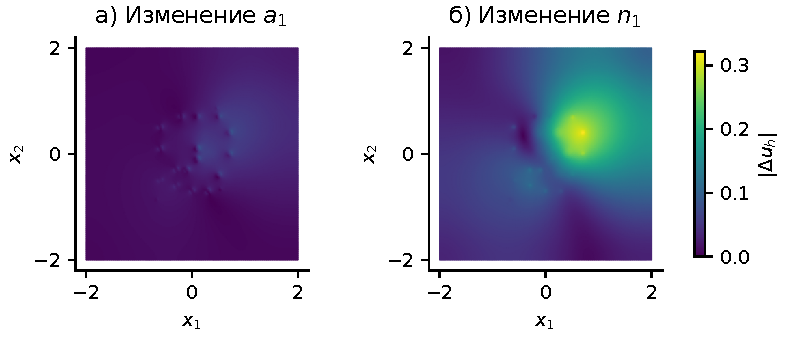
\includegraphics[width=.78\linewidth]{figures/increments.pdf}
\captionof{figure}{Модуль приращения рассеянного поля МКЭ при $\theta=\pi/8$ для двух изменений из табл.~\ref{tab:change}. Шкала одинакова для обеих карт.}
\end{localfigure}
Сеть без материальных параметров выдаёт одно и то же поле для двух сред при одинаковом направлении. Её приращение равно нулю, поэтому $E_\Delta=100\%$ в обоих опытах. Для сети с четырьмя параметрами материала получено \AlphaError\% при изменении $a_1$ и \IndexError\% при изменении $n_1$. Это оценки для двух конечных изменений относительно одной заданной среды.

\section{Заключение}
Передача двух значений $a_j$ и двух значений $n_j$ позволила одной сети восстанавливать поле при смене материала. На отложенных средах средняя погрешность составила \BestMean\% против \BlindMean\% у сети, получающей только угол. GMsFEM типа~2 с 16 локальными модами дал \GmsMean\%. На \Wins{} из 128 отдельных задач его погрешность была меньше, чем у выбранной по валидации SVD-SNO. Для каждой конфигурации использована одна инициализация сети. Эксперимент охватывает изменения четырёх скалярных параметров при заданных группах включений, $k=2$ и восьми направлениях. Для другой геометрии, анизотропного $A$ или произвольного распределения коэффициентов потребуются дополнительные расчёты.

\begingroup\small\begin{thebibliography}{9}\setlength{\itemsep}{0pt}
\bibitem{kalachikova} Kalachikova U., Vasilyeva M., Harris I., Chung E. T. Generalized Multiscale Finite Element Method for scattering problem in heterogeneous media. \emph{J. Comput. Appl. Math.} 2023. Vol.~424. 114977. \href{https://doi.org/10.1016/j.cam.2022.114977}{doi:10.1016/j.cam.2022.114977}.
\bibitem{sirovich} Sirovich L. Turbulence and the dynamics of coherent structures. Part I. Coherent structures. \emph{Quart. Appl. Math.} 1987. Vol.~45. P.~561--571. \href{https://doi.org/10.1090/qam/910462}{doi:10.1090/qam/910462}.
\bibitem{fanaskov} Fanaskov V., Oseledets I. Spectral Neural Operators. 2022, revised 2024. \href{https://arxiv.org/abs/2205.10573}{arXiv:2205.10573}.
\bibitem{sobol} Соболь И. М. О распределении точек в кубе и приближённом вычислении интегралов. \emph{Ж. вычисл. матем. и матем. физ.} 1967. Т.~7, №~4. С.~784--802.
\end{thebibliography}\endgroup
\end{document}
